\documentclass[12pt,a4paper]{extarticle}

\usepackage[czech]{babel}
\usepackage[utf8]{inputenc}
\usepackage[IL2]{fontenc}
\usepackage{amsmath}
\usepackage{amssymb}
\usepackage{mathtools}
\usepackage{graphicx}
\usepackage[margin=6mm]{geometry}
\newenvironment{amatrix}[1]{%
  \left(\begin{array}{@{}*{#1}{c}|c@{}}
}{%
  \end{array}\right)
}

\pagestyle{empty}

\newcount\pr

\parindent=0pt

% vysledky
\def\priklad#1#2{\advance\pr1 \textbf{\the\pr.} #1\par
\smallskip
#2\par \bigskip}

% zadani
%\def\priklad#1#2{\advance\pr1\nointerlineskip\vbox to.0588\vsize{\vss\hbox{{\Large\bfseries \tym\ifnum\pr<10 0\fi\the\pr}\quad \vtop{\hsize=.9\hsize\relax#1}}\vss}\vfil}

\def\printtym#1{\pr0\def\tym{#1}\priklady\vfill\newpage}

\begin{document}

\def\priklady{%
\priklad{Kolik schodů musí člověk vystoupat na hlavním schodišti z přízemí do 3. patra? (Počítá se i \uv{závěrečný schod})}{81}

\priklad{Nalezněte všechna reálná řešení $x^2 - \sqrt2 x + \sqrt 3 x - \sqrt 6 = 0$.}{$\sqrt2, -\sqrt3$}

\priklad{Vyřešte kongruenci $12x \equiv 14 \pmod{47}$.}{$x \equiv 9 \pmod{47}$}

\priklad{Kolik hran bude mít strom s 50 vrcholy?}{49}

\priklad{Spočtěte determinant $\displaystyle\begin{vmatrix}1&-6&5 \\ 2&2&5 \\ -1&-4&1\end{vmatrix}$.}{34}

\priklad{Nalezněte příklad skóre, které budou mít hned \emph{tři} neisomorfní grafy, a sestrojte ony grafy.}{Připojíme vrchol někam na cestu.}

\priklad{Nalezněte polynom 2. stupně $f$, který bude splňovat $f(1)=1$, $f(0)=-4$, $f(-2)=-2$}{$2x^2 + 3x - 4$.}

\priklad{Kolik koster má tento graf: $\vcenter{\hbox{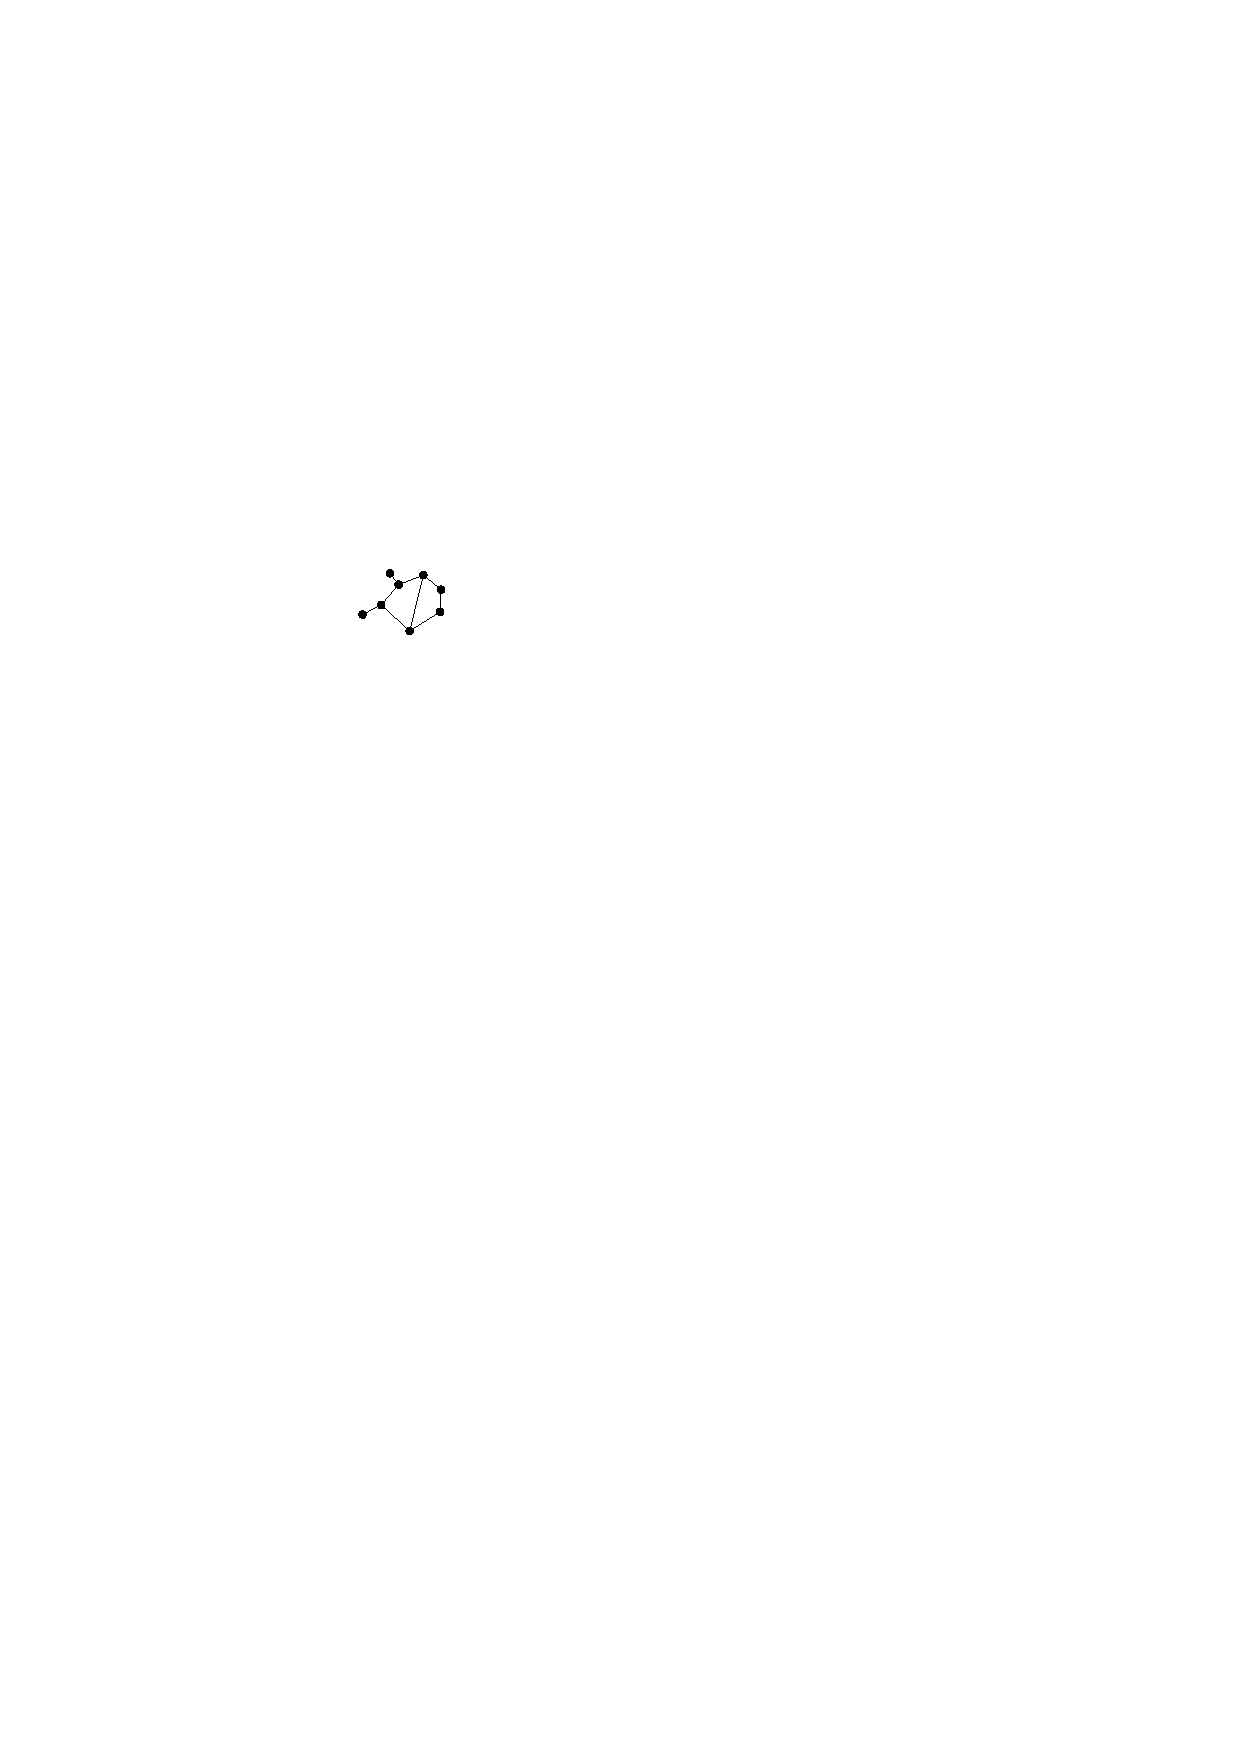
\includegraphics{pagraf.pdf}}}$ ?}{15}

\priklad{Hrajeme hru \uv{odeber 1, 2, či 4 sirky, kdo nemůže, prohrál}. Určete hodnoty SG funkce pro stavy, kdy je na stole 0--9 sirek.}{0, 1, 2, 0, 1, 2, 0, 1, 2, 0}

\priklad{Sestrojte alespoň dva navzájem neisomorfní grafy se skóre $(1, 1, 3, 3, 3, 3)$.}{$K_4$ + $K_2$, cesta délky 5 s napojeným vrcholem doprostřed}

\priklad{Vyřešte soustavu kongruencí $3x\equiv 4\pmod{11}$, $2x\equiv 3 \pmod{5}$.}{$x \equiv 49 \pmod{55}$}

\priklad{Nalezněte všechna řešení soustavy rovnic $\begin{amatrix}{3}0&1&1& 3 \\1&2&3& 2 \\1&1&2& -1\end{amatrix}$.}{$\{(-4+t, 3+t, -t)\mid t \in \mathbb R\}$}

\priklad{Převeďte číslo 2022 do soustavy o základu 3.}{2202220}

\priklad{Nalezněte polynom 3. stupně, jehož kořeny budou $2$, $3$ a $-1$. Uveďte ho ve tvaru $ax^3 + bx^2 + cx + d$.}{$x^3-4 x^2+x+6$}

\priklad{Spočtěte determinant $\begin{vmatrix}\sqrt2&\sqrt3&\sqrt6 \\ \sqrt6&-\sqrt2&\sqrt3 \\ \sqrt3&\sqrt2&-\sqrt2\end{vmatrix}$}{$12+8\sqrt2 + \sqrt3$}

\priklad{Nalezněte všechna reálná řešení $x^3-4 x^2+5 x-2 = 0$.}{$1, 2$}

\priklad{Na každou stěnu dvacetistěnu přilepíme (pravidelný) čtyřstěn o stejné délce hrany. Kolik bude mít vzniklé těleso vrcholů/hran/stěn?}{32/90/60}

\priklad{Kolik vyučujících celkem sídlí ve sborovně (\uv{multikabinetu}) v 1. patře?}{19}

\priklad{Nalezněte inverzní prvek k $6$ modulo $43$.}{36}

\priklad{Určete zbytek $7^{777}$ po dělení $16$.}{7}

\priklad{Nalezněte všechna reálná $x$ splňující $\begin{vmatrix}8&6&4 \\ x&5&5 \\ 7&x&x-2\end{vmatrix} = 0$}{1, 5}

\priklad{Vyřešte soustavu kongruencí $x\equiv1 \pmod2$, $x \equiv1 \pmod3$, $x \equiv 7\pmod{17}$.}{$x \equiv 7 \pmod{102}$}

\priklad{Nalezněte všechna reálná řešení $x^4-3 x^3-10 x^2+3 x+9=0$.}{$\pm 1, \frac32(1\pm\sqrt5)$}

\priklad{Obarvěte vrcholy grafu co nejméně barvami, aby spojené vrcholy měly různou barvu: $\vcenter{\hbox{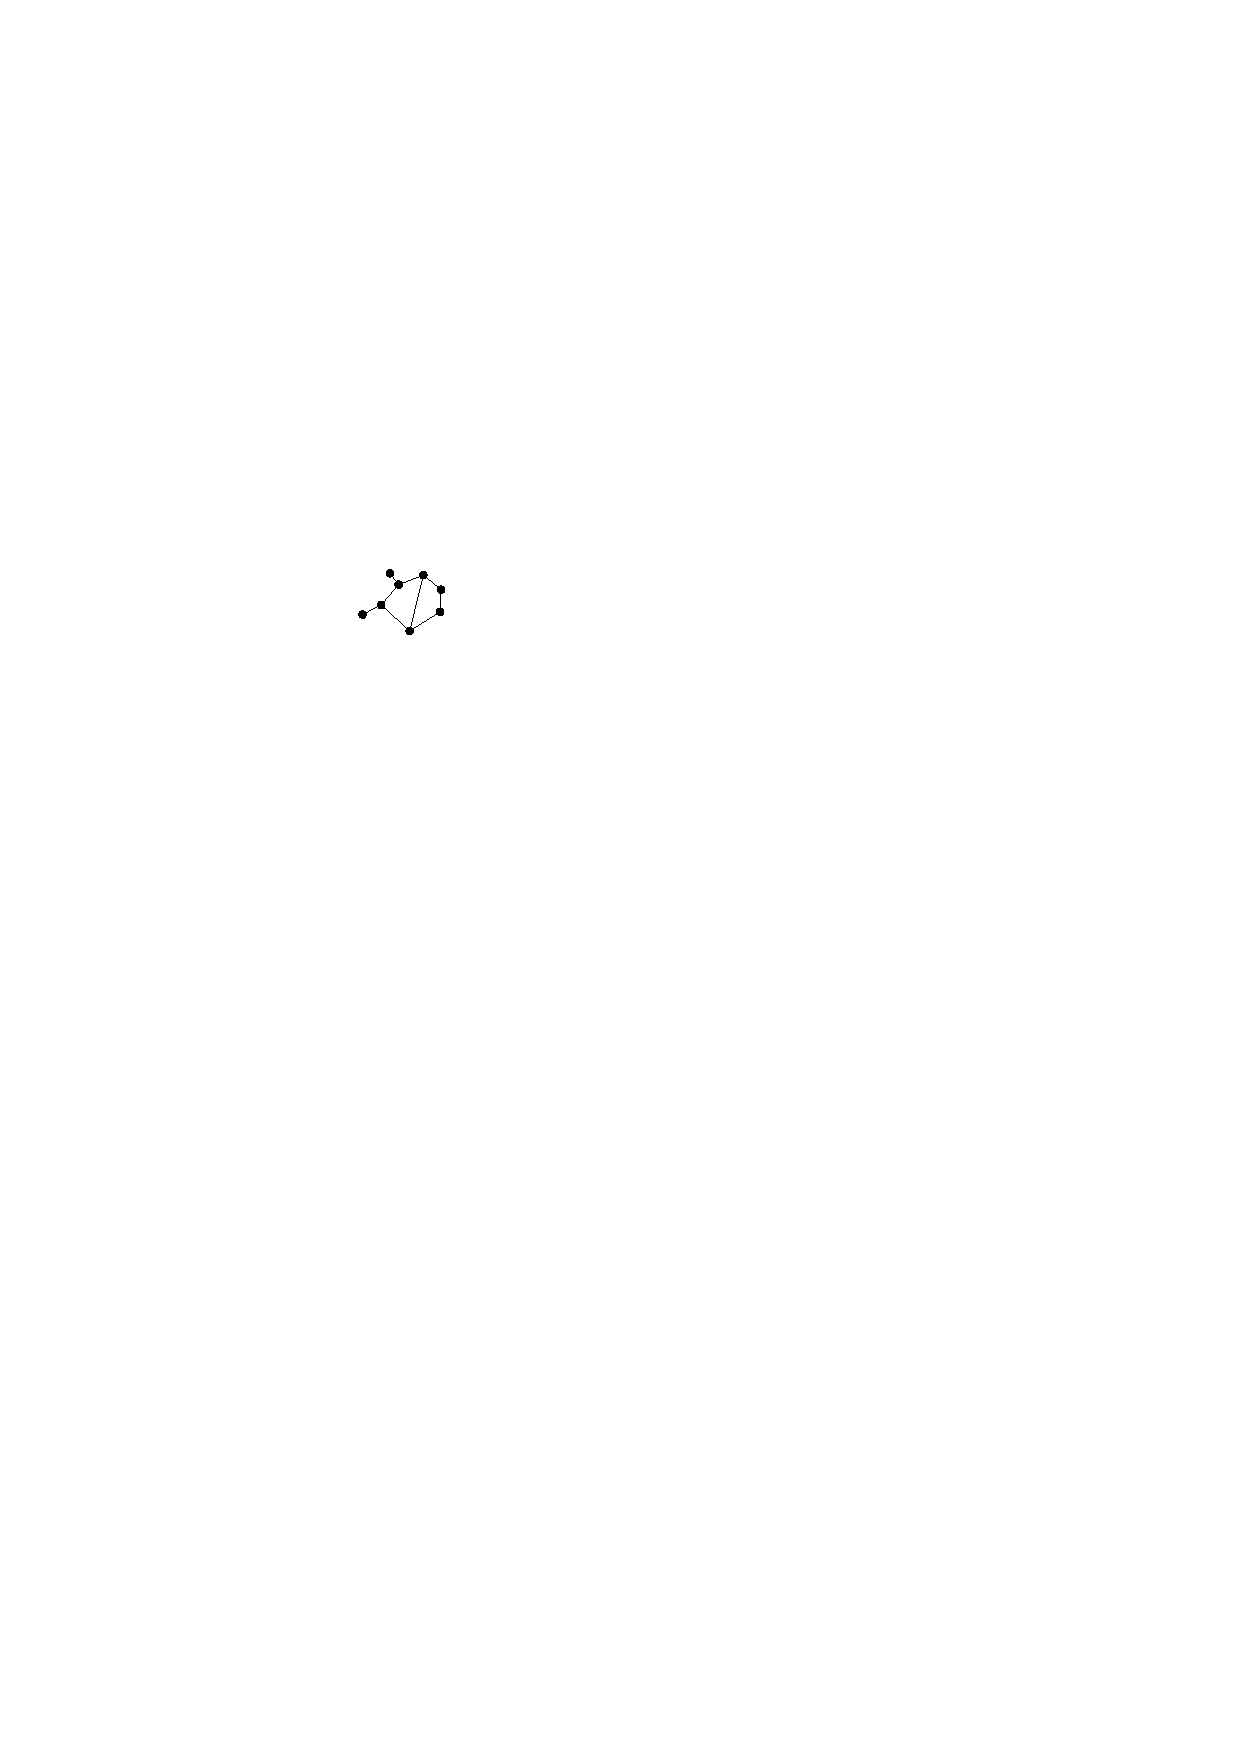
\includegraphics{pagraf.pdf}}}$}{jde to dvěma}

\priklad{Spočtěte determinant $\left|\begin{smallmatrix}1&1&1&1 \\ 1&2&3&4 \\ 1&3&6&10 \\ 1&4&10&20\end{smallmatrix}\right|$.}{1}

\priklad{Spočtěte $\varphi(63000)$.}{14400}

\priklad{Nalezněte všechny možné cifry $x$ takové, že číslo $123456789x$ bude dělitelné $11$.}{5}

\priklad{Stěny jistého (konvexního) tělesa tvoří pouze čtverce a pravidelné šestiúhelníky, přičemž v každém vrcholu se setkávají dva šestiúhelníky a jeden čtverec. Kolik stěn jakého typu má těleso?}{6 čtverců, 8 šestiúhelníků}

\priklad{Pro která všechna přirozená $n$ bude mít číslo $2022$ zapsané v soustavě o základu $n$ přesně $4$ cifry?}{7--12}

\priklad{Sestrojte graf, jehož skóre tvoří dvacet čtyřek.}{Čtyřikrát $K_5$}

\priklad{Určete poslední dvě cifry čísla $2^{1000}$.}{76}

\priklad{Převeďte z šestnáctkové soustavy do dvojkové číslo DEADBEEF.}{11011110\,10101101\,10111110\,11101111}

\priklad{Hrajeme standardní hru \uv{odeber libovolně sirek z jedné hromádky, kdo nemůže, prohrál}, přičemž na stole jsou hromádky o velikostech 29, 20, 7, 17, 1. Popište všechny možné tahy, které můžeme udělat, abychom určitě vyhráli.}{$29\to3$, $20\to10$, $17\to15$}

}

\printtym{A}
%\printtym{B}
%\printtym{C}
%\printtym{D}
%\printtym{E}
%\printtym{F}




\end{document}